Dieses Kapitel beschäftigt sich damit, wie man Programme auf Data Races überprüft.\\
\\
Race Detection Programme zur Überprüfung von Thread Safety Problemen werden in der Literatur in zwei Kategorien unterteilt: Dynamische und Statische Race Detection. 

Statische Race Detection analysiert dabei den Quell-, beziehungsweise Byte Code des Programms, ohne es auszuführen. Die Dynamische Methode hingegen führt das Programm aus und analysiert dieses während der Laufzeit. Unterscheiden wird bei der Dynamischen Race Detection zwischen der Erkennung durch eine \acs{HB} Beziehung und den Lockset Algorithmus \cite[vgl.][4]{erickson_effective_nodate}. "Despite significant advances in static race detection, state-of the-art race detection tools are still predominantly dynamic" \cite[308]{naik_effective_nodate}.

\section{Dynamische Race Detection durch die Happens Before Beziehung}

In dieser Sektion wird Dynamische Race Detection durch die \acs{HB} Beziehung behandelt. Eine \acs{HB} Beziehung liegt vor, wenn bei zwei Aktionen A und B eine Verzögerung in A eine Verzögerung in B verursacht. Wenn keine \acs{HB} Beziehung vorliegt, kann man daraus ein Thread Safety Problem folgern \cite[vgl.][163]{li_efficient_2019}. Um die Wahrscheinlichkeit für das Vorkommen dieser Beziehung zu erhöhen, verzögern beide Algorithmen das Programm.  

\subsection{Data Collider}

Data Collider ist einer der Algorithmen, welcher die \acs{HB} Beziehung ausnutzt, um Data Races zu finden. Dazu benutzt Data Collider zunächst einen Sampling Algorithmus um einen kleinen Teil an Speicher Zugriffen nimmt und diese speichert. Jene Speicherzugriffe werden daraufhin an die Konflikt Erkennung weiter gegeben, um Data Races zu finden. Zuletzt verwendet Data Collider mehrere Heuristiken, um gutartige Data Races zu entfernen \cite[vgl.][6]{erickson_effective_nodate}.  

\subsubsection*{Sampling Algorithmus}

Data Collider nimmt den zu Analysierenden Programm Code als Binärdatei und schreibt alle Stellen an denen der Speicher angesprochen wird in ein Sampling Set. Aus dem Sampling Set entfernt werden dabei Anweisungen die nur den Threadlokale Stack Speicherplätze ansprechen und Synchronisierungsanweisungen. Data Collider nimmt daraufhin proben aus dem Sampling Set in dem es Breakpoints einfügt, die dann genutzt werden um Konflikte zu erkennen \cite[vgl.][6]{erickson_effective_nodate}. 

\subsubsection*{Konflikterkennung}

Konflikterkennung entsteht bei Data Collider entweder durch Data Breakpoints oder durch Reapeated Reads \cite[vgl.][7]{erickson_effective_nodate}. Data Breakpoints funktionieren über die vier von einem CPU der x86 Architektur gegebenen Data Breakpoint Register. Wenn ein Zugriff auf den Speicher eine Schreiboperation ist, sagt Data Collider dem Prozessor, dass dieser eine Falle aufstellen soll für diese Speicherstelle. Die Ausführung dieses Threads wird dann verzögert. Bei einer intialen Leseoperation wird die Falle nur ausgelöst, wenn auf die Speicherstelle mit einer Schreiboperation zugegriffen wird \cite[vgl.][7-8]{erickson_effective_nodate}.\\
\\
Sobald Data Collider keine Breakpoint Register mehr hat, greift der Algorithmus auf Repreated Reads zurück. Falls ein Zugriff auf den Speicher gemacht wird, wird der Thread wieder verzögert. Währenddessen wird die ganze Zeit überprüft, ob sich die Speicherstelle verändert. Wenn diese verändert wird, liegt ein Data Race vor. Jedoch ist es schwierig herauszufinden, durch welche Stelle das Data Race verursacht wurde \cite[vgl.][7-8]{erickson_effective_nodate}. 

\subsubsection*{Umgang mit gutartigen Datenabweichungen}

"Research on data-race detection has amply noted the fact that not all data races are erroneous" \cite[8]{erickson_effective_nodate}. Diese Data Races müssen aus der Ausgabe der gefundenen Bugs entfernt werden. Dazu benutzt Data Collider drei Muster, um dies zu erkennen: Statische Zähler, Safe Flag Updates und Spezielle Variablen \cite[vgl.][8]{erickson_effective_nodate}.\\
\\
Statische Zähler sind da, um diverse Statistiken über das Programm zu machen. Statische Zähler welche Write Only sind werden als gutartig markiert \cite[vgl.][8]{erickson_effective_nodate}. Safe Flag Updates besteht darin, dass ein Thread ein Flag Bit in einem Speicherplatz liest, während ein anderer Thread ein anderes Bit in demselben Speicherplatz aktualisiert. Jedoch gehen bei Schreib-Schreib Konflikten hierbei Informationen verloren, somit werden diese weiterhin beachtet \cite[vgl.][8]{erickson_effective_nodate}. In Windows Kernel, für den Data Collider gemacht wurde, gibt es Spezielle Variablen, bei denen Data Races erwartet werden und kein Problem darstellen. Diese Stellen werden durch eine Datenbank an Speziellen Variablen von Data Collider nicht beachtet \cite[vgl.][8]{erickson_effective_nodate}.

\subsection{TSVD}

\ac{TSVD} benutzt Near-Miss Tracking, um potentielle Stellen Paare für Data Races zu finden. Zudem wird \acs{HB} Tracking genutzt, welches durch Verzögerungen die Wahrscheinlichkeit für ein Data Race erhöht \cite[vgl.][163]{li_efficient_2019}.

\subsubsection*{Near-Miss Tracking}

In einem Programm nennt \acs{TSVD} ein Paar an Programmstellen gefährlich, wenn zwei verschiedene Threads auf das selbe Objekt zugreifen und eine der Operationen, die ausgeführt wird, und die Zeit zwischen den Zugriffen unter einem bestimmten Schwellenwert ist \cite[vgl.][168]{li_efficient_2019}.  

\subsubsection*{Wo wird Verzögert?}

\acs{TSVD} benutzt ein Trap Set, um gefährliche Paare zu speichern, bei denen potentiell Data Races entstehen können. Der Algorithmus will Near-Misses zu wahren Konflikten machen, also werden Near-Misses in das Trap Set hinzugefügt. Aus dem Trap Set werden Paare entfernt, die entweder einen wahren Konflikt ausgelöst haben oder eine \acs{HB} Bezeihung zueinander haben \cite[vgl.][167]{li_efficient_2019}.

\subsubsection*{Wann wird Verzögert?}

Die Planung und Injektion sind bei \acs{TSVD} in einem Durchlauf des Programms. Zudem werden mehrere Testdurchläufe gemacht, da die Möglichkeit besteht, dass gefährliche Paare nie in der Nähe von einander aufgerufen werden. Das Trap Set, welches \acs{TSVD} speichert, wird in einen Trap File geschrieben und beim nächsten Durchlauf als initial Wert für das Trap Set genutzt \cite[vgl.][169]{li_efficient_2019}.  


\subsubsection*{Algorithmus}

%\begin{comment}
\begin{lstlisting}[language=Java,frame=tb,caption={\acs{TSVD} Trap Mechanism}, label={lst:TSVD}, numbers=left, stepnumber=1,  captionpos=b, tabsize=4]
OnCall (thread_id, obj_id, op_id) { 
     check_for_trap(thread_id , obj_id , op_id) 
     if (should_delay(op_id)) {
         set_trap(thread_id, obj_id, op_id)
         delay()
         clear_trap(thread_id, obj_id, op_id)
    }
}
\end{lstlisting}
%\end{comment}

In \ref{lst:TSVD} dargestellt ist der Algorithmus, der verwendet wird, um Thread Safety Verstöße in \acs{TSVD} zu finden \cite[Figure 5,][166]{li_efficient_2019}. Das Prinzip des Algorithmus ist eine Falle für Thread Safety Verstöße zu stellen und zu warten, ob ein anderer Thread die Falle auslöst. \\
\\
Die Funktion \texttt{OnCall} nimmt als Parameter die Id des Threads, von dem diese ausgelöst wird, die Id vom Objekt, auf welches zugegriffen wird, und die Operation Id, also welche Operation auf dem Objekt ausgeführt wird. Sobald die Methode \texttt{OnCall} von einem Thread auf ein Objekt aufgerufen wird, wird in Zeile 3 überprüft, ob eine Falle gesetzt werden soll. Wenn diese gesetzt werden soll, so wird dies umgesetzt und eine bestimmte Zeit gewartet bis die Falle aufgelöst wird. Wenn nun ein anderer Thread \texttt{OnCall} auf das selbe Objekt aufruft und einer der Operationen eine Schreib Operation war, gilt die Falle als ausgelöst und vom Programm wird dieser Bug zurück gegeben \cite[vgl.][166]{li_efficient_2019}.

\subsubsection*{Implementation}

Die Implementation dieses Algorithmus wurde für .NET Applikationen gemacht (\url{https://github.com/microsoft/TSVD}). Dabei wurde das Programm aufgeteilt in den \acs{TSVD} Instrumenter und \acs{TSVD} Runtime. \\ 
\\
Der Instrumenter ist dabei ein \ac{CLI} Tool oder in Visual Studio ein Post-Build Step. Als Eingabe nimmt das Programm dabei die Binärdatei eines Programms und eine Liste an Thread unsicheren \ac{API}s. Der Instumenter ersetzt dann die Aufrufe auf die Thread unsicheren \acs{API}s mit Proxy Aufrufen. Wie diese Proxy Aufrufe funktionieren, ist in \ref{lst:TSVDImpl} dargestellt. \cite[vgl.][170]{li_efficient_2019}. \acs{TSVD} Runtime hingegen implementiert die \texttt{OnCall} Methode und protokolliert den Kontext, wenn ein Bug gefunden wird \cite[vgl.][170-171]{li_efficient_2019}.
\\
%\begin{comment}
\begin{lstlisting}[language=Java,frame=tb,caption={\acs{TSVD} Proxy Aufrufe}, label={lst:TSVDImpl}, numbers=left, stepnumber=1, captionpos=b, tabsize=4]
// (a) Original code
List <int> listObject = new List <int>();
listObject.Add(15); 
      
// (b) Instrumented code 
List <int> listObject = new List <int>(); 
int op_id = GetOpId(); 
Proxy_123(listObject , 15, op_id); 
     
// (c) Proxy method
void Proxy_123 ( Object obj , int x ,int op_id ) { 
    var thread_id = GetCurrentThreadId (); 
    var obj_id = obj.GetHashCode(); 
    OnCall(thread_id , obj_id , op_id); 
    obj.Add(x);
}
\end{lstlisting}
%\end{comment}

\subsection*{Vergleich TSVD mit Data Collider}

%\begin{comment}
\begin{figure}[ht]
    \centering
    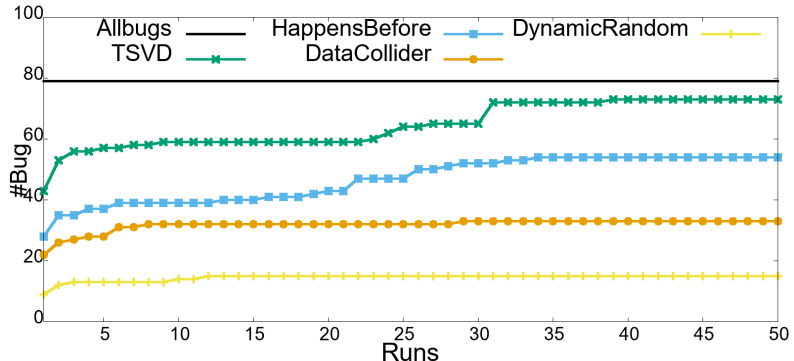
\includegraphics[width=0.8\textwidth]{gfx/TSVDvDataCollider.png}
    \caption{Vergleich TSVD mit Data Collider \cite[173]{li_efficient_2019}}
    \label{fig:TSVDvDataCollider}
\end{figure}
%\end{comment}

In dieser Sektion wird \acs{TSVD} mit Data Collider verglichen. \acs{TSVD} hat in der ersten Runde 42 Bugs und nach zwei Runden 11 weitere Bugs gefunden, während Data Collider signifikant weniger Bugs gefunden hat, was in \ref{fig:TSVDvDataCollider} erkannt werden kann.